\section{Background and Related Work}\label{sec:background}

This paper aims at designing a biometric-based challenge-response authentication system that can verify legitimate user(s) and reject attackers.
Our system utilizes a Leap Motion controller, a 3D motion sensor, to track the user's 3D handwriting, based on which we verify whether what a user write matches what is asked for. Then we perform feature extraction and user authentication. 
%The proposed system consists of a training stage, when it learns each user's writing style from a set of writing samples, and a testing stage, when it applies the trained classifier for identifying a user based on a new writing input.

In this section, we define attack models, introduce the Leap Motion controller, and discuss the related work. 



\subsection{Background}
\label{sec:bg}

\subsubsection{Attack Model}
We assume that the system is used in a well controlled environment and attackers have no physical access to the hardware (i.e., the Leap Motion) nor the software (e.g., the operating systems or databases). Second, the communication path between the Leap Motion and a computer is secure so that no attackers can hijack or inject motion data in between. Attackers can only attempt to impersonate users by writing in front of a Leap Motion controller while mimicking other users. 
we consider the following \jing{two} types of attack models. 

%\begin{itemize}
1) \textbf{Non-Observing attackers} try to imitate a legitimate user without any knowledge of the victim's handwriting style, and hope to be identified as the victim with random writings. In particular, Non-Observing attackers can be either an insider that has enrolled in the \CiT system or an impostor without enrollment.  


2) \textbf{Observing attackers} are better informed and they could have visually observed the victim's writing process, % in front of a Leap Motion, by shoulder surfing,  
and have viewed finger trajectories of the victim's handwriting displayed on a computer screen.  


%3) \textbf{Naive robot arm attackers} are introduced to emulate a super human who can precisely reproduce the recorded finger movements, so that we can evaluate the upper bound of the impact of shoulder surfing. 
%%Given that a robot arm attacker can repeatedly replay the same  recorded motion, our system can perform a content check to detect such scenarios, i.e., utilizing similarity comparison or content recognition using online handwritng recognition techniques~\cite{Tappert90}.  
%\jingnew{Since \CiT adapts CR mechanism,  the naive robot arm has to write different content to take the challenge. }
%We assume that a naive robot-arm can record some observations of the victim and split writing trajectories that correspond to each letter, and synthesize the writing of the new word by sequentially linking the writing trajectory of each letter of the required string. \jingnew{We assume the robot arm does not have unlimited access to the victim, thus it is not capable of get  transitions between letters, which demands the recording of $26\times26$ types of transitions. }





\subsubsection{Leap Motion Controllers}

Leap Motion is a motion sensor connected to a computer via a USB port, and it can track the motion of human hands and all ten fingers in the 3D space. Compared to the Microsoft Kinect, the Leap Motion tracks hands including fingers (e.g., finger tips) in a much higher precision but in a smaller space. 
In particular, it can periodically provide
information on finger width, length and motion velocity.   
Such information reflects the user's hand-motion kinematics, from which we can 
recognize the user's handwriting style.

\jingnew{Leap Motion is equipped with two cameras and three infrared LEDs~\cite{leapBlog}.} The 3D positions of fingers are derived by combining their 2D positions on the image frames taken by the two cameras and depth measured by the infrared lights. 
As a user write in front of a Leap Motion (as shown in Figure~\ref{fig:leap}) using one of his finger, % shows a leap motion controller in front of a computer screen, on which the tracking of a fingertip is displayed in real time.
a trajectory of the finger is formed by connecting fingertip positions sequentially and is displayed on the screen.
Leap Motion uses the Cartesian coordinate system and can track the fingers in a 3D space of an inverted pyramid centered on the device, and the effective range is approximately 25 to 600 mm above the device (1 inch to 2 feet)~\cite{LeapOnlineOverview,leapBlog}.
Based on our measurements, it can track the position and velocity of the human fingertips at a rate of around $114$ frames per second and with a spatial resolution of $0.01$mm.

%\jingnew{Since its release in July 2013, Leap Motion has hundreds of applications on its app store and was used to operate computers by 3D hand motion. It is also an option for free hand TV control application~\cite{Zaiţi2015:TVcontrol}  and possible Virtual Reality related applications~\cite{LeapOrion}. }
%%For example, the gesture of a ``hand swipe" can be used to turn a page when reading an electronic book.  Leap Motion controllers also have been endorsed by computer manufactures, e.g., HP Envy 17 Leap Motion Special Edition.  
%In summary, Leap Motion is gaining its popularity and is ideal for capturing handwriting motion. 

%has already gained its popularity as a new input device, and is ideal for capturing handwriting motion in our system. 




\begin{figure*}[!bhp]
\vspace{-0mm}
\centering
\begin{tabular}{|cc|cc|}
\hline
%\vspace{1mm}
      & User 1 & User 2 &
\\ \hline %\hline %\vspace{1mm}

{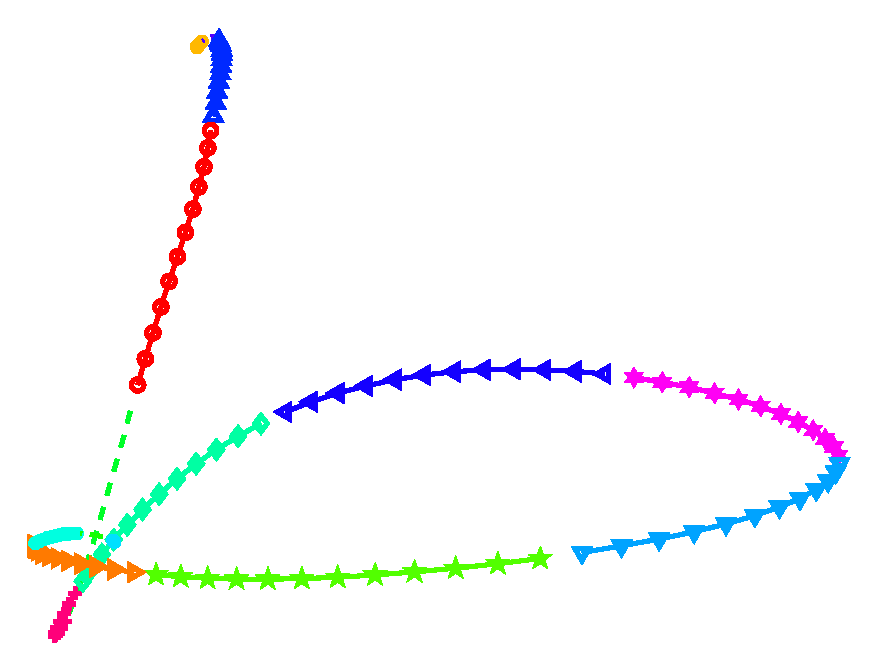
\includegraphics[width=.3\columnwidth]{./Graphic/Pic_words_forSystemSection/user_2_bphmn_2_at_3th_component.eps}}
&{\includegraphics[width=.55\columnwidth]{./Graphic/Pic_words_forSystemSection/user1_b.eps}}  
&{\includegraphics[width=.55\columnwidth]{./Graphic/Pic_words_forSystemSection/user2_b.eps}} &{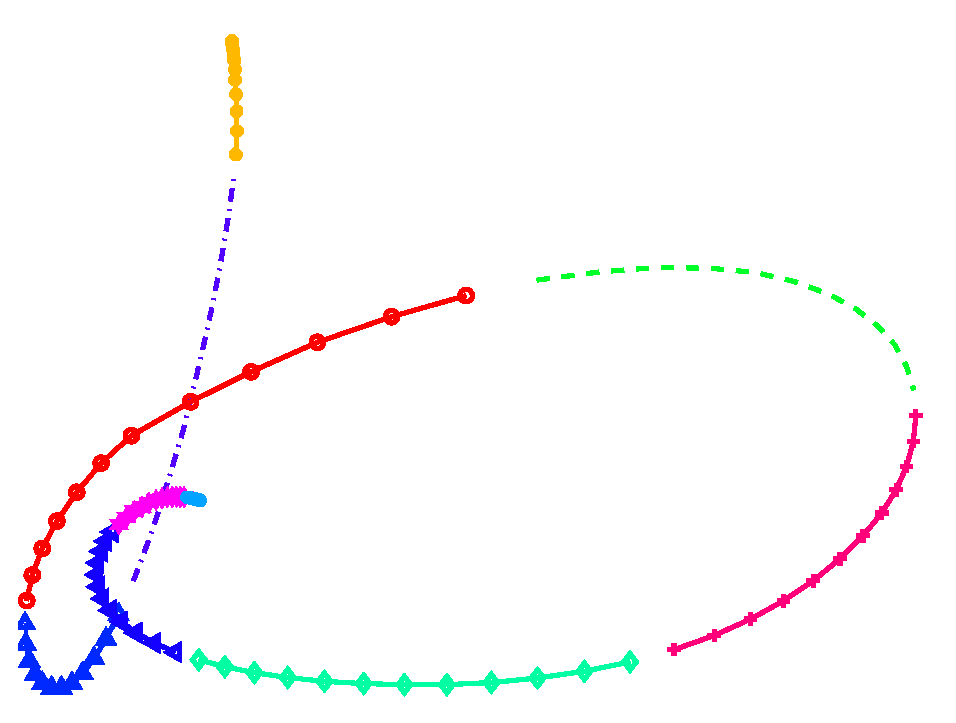
\includegraphics[width=.3\columnwidth]{./Graphic/Pic_words_forSystemSection/user_1_bphmn_2_at_5th_component.eps}} 

\\ \hline %\vspace{1mm}

 %LP.pdf
{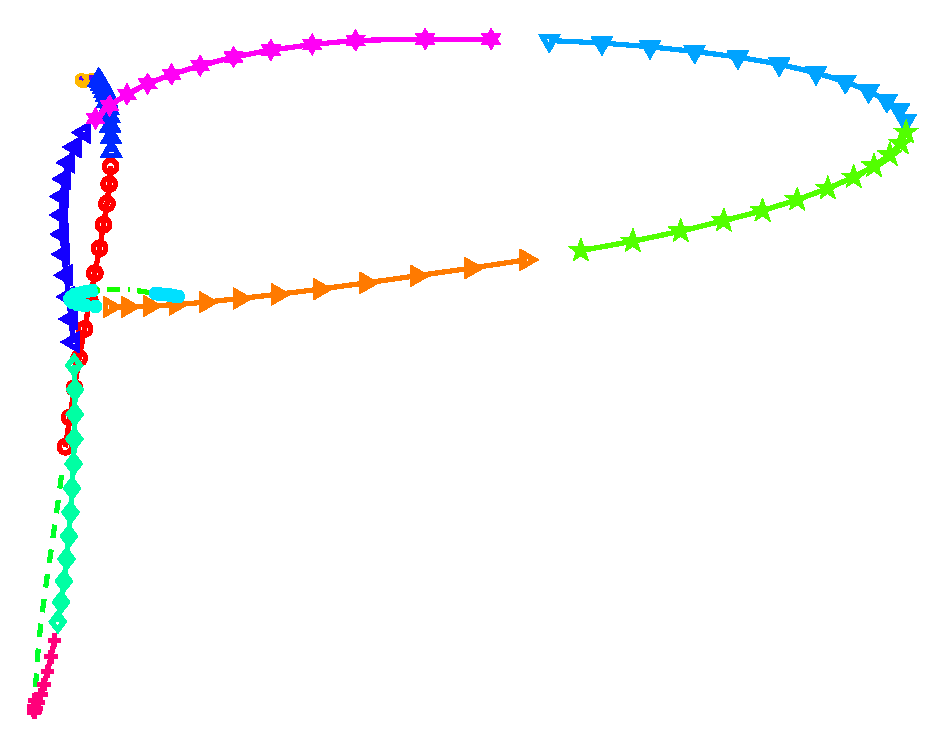
\includegraphics[width=.3\columnwidth]{./Graphic/Pic_words_forSystemSection/user_2_bphmn_2_at_4th_component.eps} }
&{\includegraphics[width=.55\columnwidth]{./Graphic/Pic_words_forSystemSection/user1_p.eps} }%LP.pdf
&{\includegraphics[width=.55\columnwidth]{./Graphic/Pic_words_forSystemSection/user2_p.eps}}
&{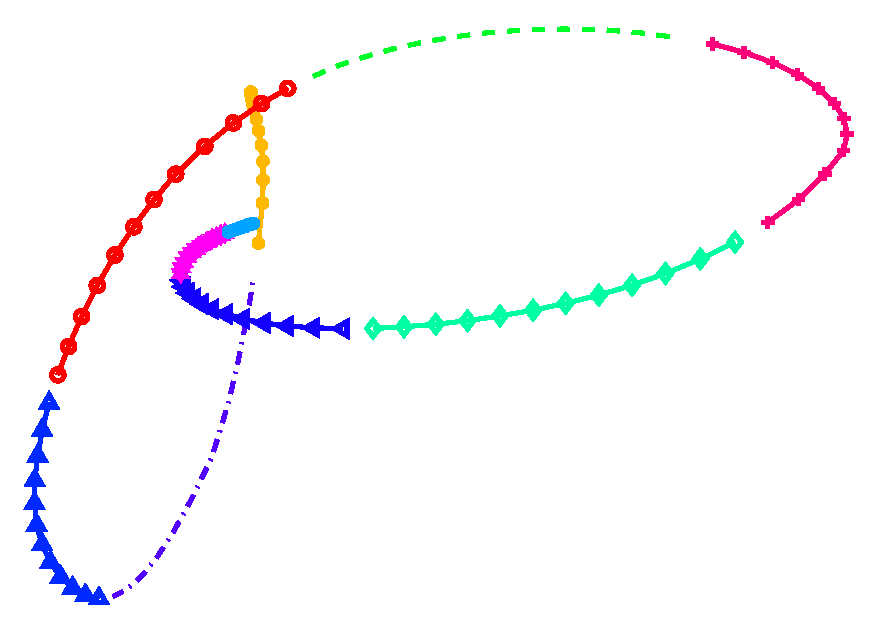
\includegraphics[width=.3\columnwidth]{./Graphic/Pic_words_forSystemSection/user_1_bphmn_2_at_8th_component.eps}} 
 \\ \hline 
 %\hline 
%
%
%% 
%%{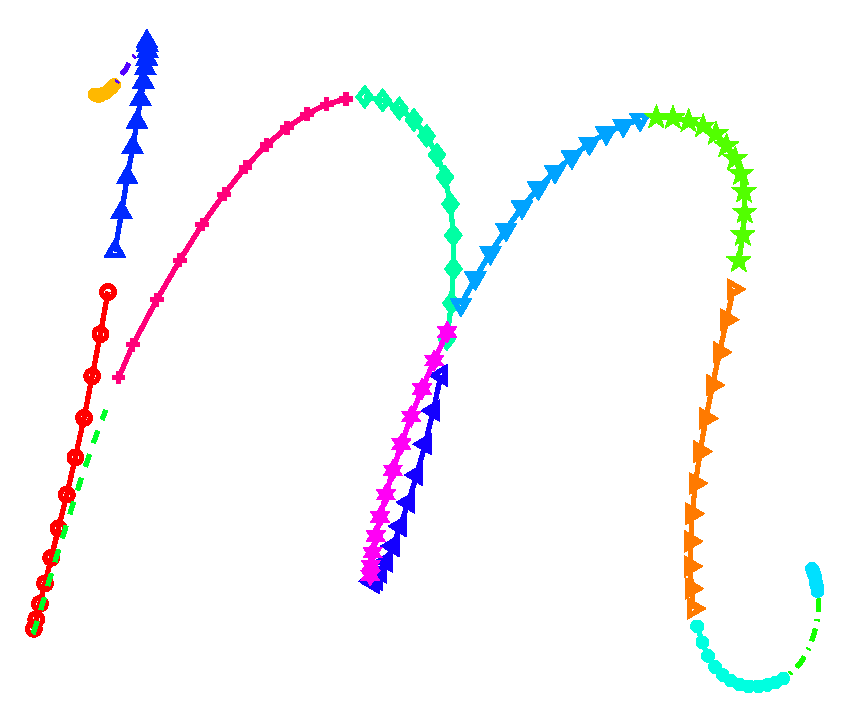
\includegraphics[width=.2\columnwidth]{./Graphic/Pic_words_forSystemSection/user_2_bphmn_1_at_5th_component.eps}}
%%&{\includegraphics[width=.5\columnwidth]{./Graphic/Pic_words_forSystemSection/1_m.eps}} 
%%&{\includegraphics[width=.5\columnwidth]{./Graphic/Pic_words_forSystemSection/2_m.eps}}  &{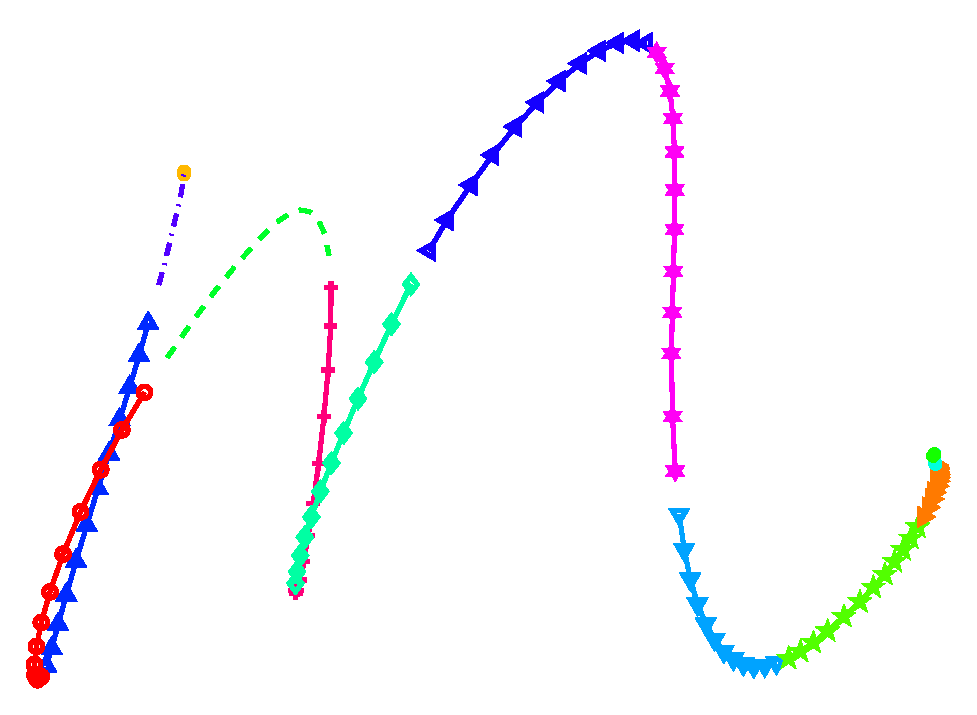
\includegraphics[width=.2\columnwidth]{./Graphic/Pic_words_forSystemSection/user_1_bphmn_1_at_8th_component.eps}} \\  \hline %\vspace{1mm}
%
%{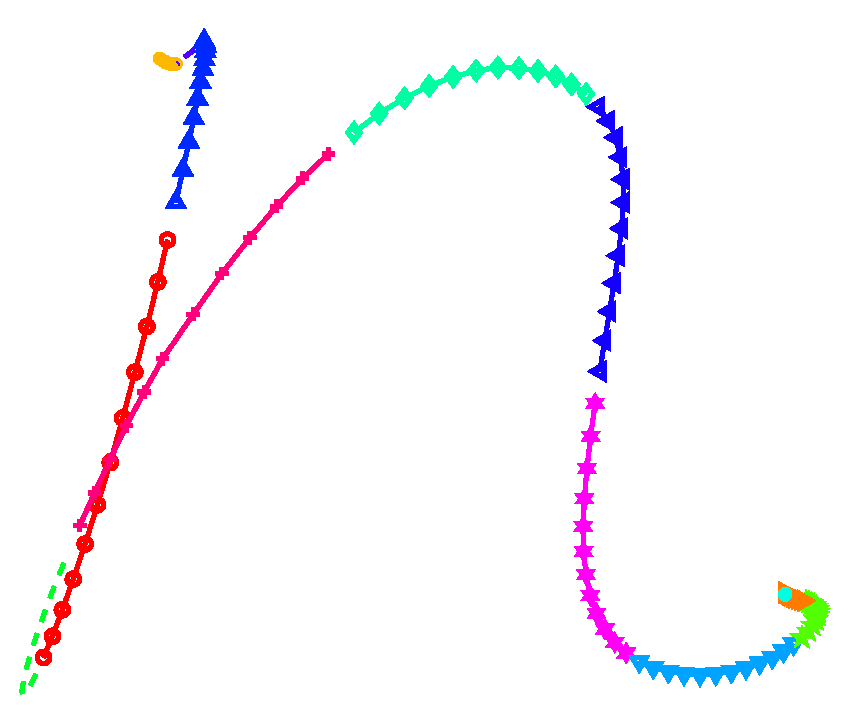
\includegraphics[width=.2\columnwidth]{./Graphic/Pic_words_forSystemSection/user_2_bphmn_1_at_6th_component.eps} } 
%&{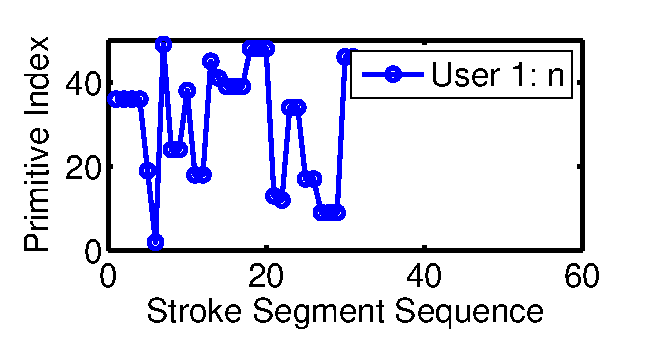
\includegraphics[width=.5\columnwidth]{./Graphic/Pic_words_forSystemSection/user1_n.eps}}
%&{\includegraphics[width=.5\columnwidth]{./Graphic/Pic_words_forSystemSection/user2_n.eps}} 
%&{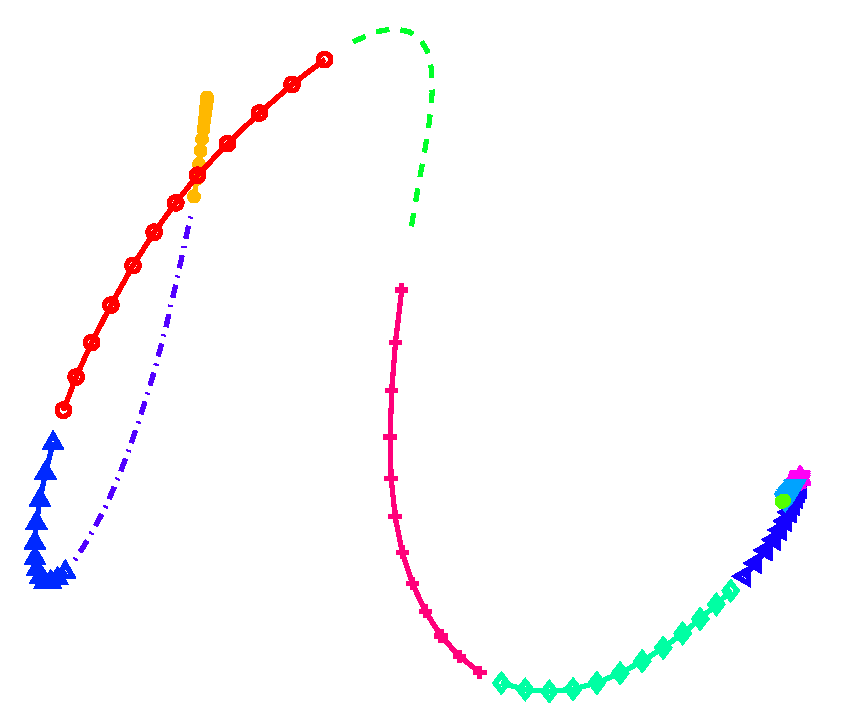
\includegraphics[width=.2\columnwidth]{./Graphic/Pic_words_forSystemSection/user_1_bphmn_1_at_9th_component.eps}} \\ \hline %\vspace{1mm}
%
%{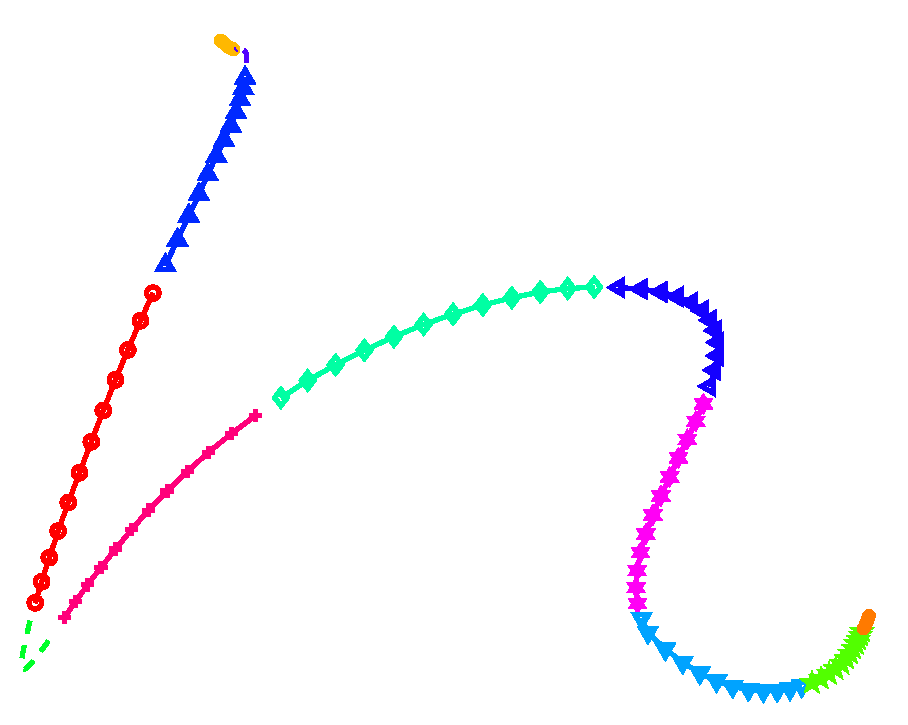
\includegraphics[width=.2\columnwidth]{./Graphic/Pic_words_forSystemSection/user_2_bphmn_1_at_10th_component.eps} }
%&{\includegraphics[width=.5\columnwidth]{./Graphic/Pic_words_forSystemSection/user1_h.eps}}
%&{\includegraphics[width=.5\columnwidth]{./Graphic/Pic_words_forSystemSection/user2_h.eps}}  
%&{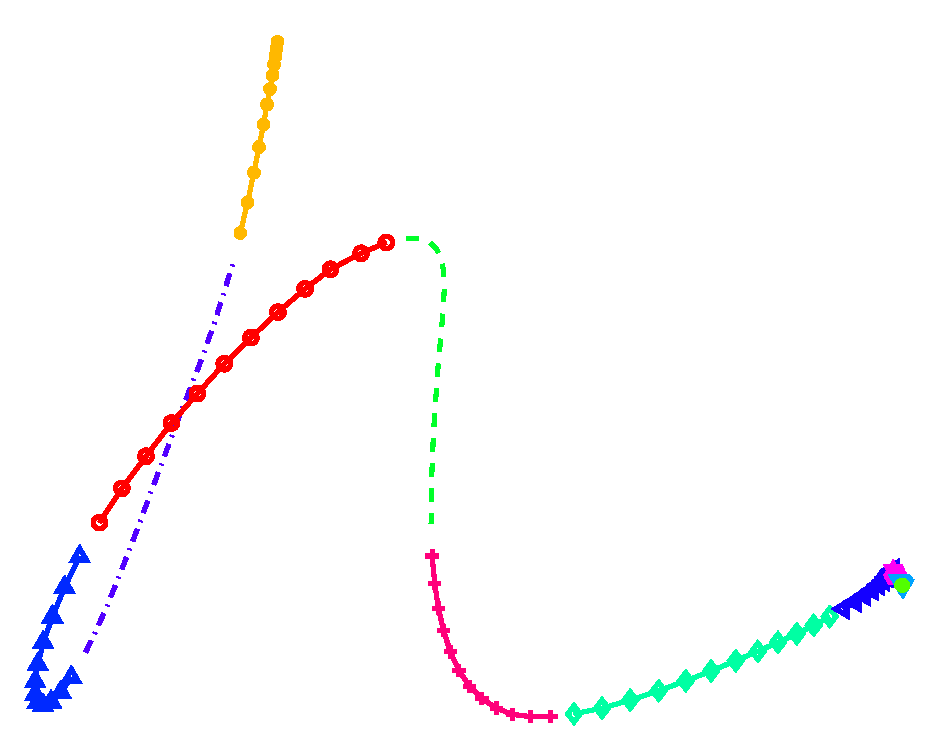
\includegraphics[width=.2\columnwidth]{./Graphic/Pic_words_forSystemSection/user_1_bphmn_1_at_4th_component.eps}} 
%\\ \hline%LP.pdf

\end{tabular}
\caption{{\jing{An illustration that characters written by the same user exhibit similarity while the ones by different users exhibit difference. We use 50 types of stroke segments (i.e., primitives) that consists of 12 continuous frames for illustration. The motion trajectories are divided into stroke segments, and the plots show the primitive-index ($y$-axis) change over time ($x$-axis). Plots with similar profiles represent the similarities of the handwriting style. 
Stroke segments (denoted by different colors on the characters) of \texttt{b} and \texttt{p} from the same user (either User 1 or User 2) show similar patterns, i.e., similar sequences of primitive indices, but the stroke segment sequences from the different users of the same letter (e.g.,  \texttt{b} or \texttt{p}) show distinguished patterns.
%Stroke segments (denoted by different colors on the characters) of `b' and `p' from the same user (either User 1 or User 2) show similar patterns in sequence donated by primitive indices, but the stroke segment sequences from the different users of the same letter `b' behave differently. %The observations also hold for `n' and `h'. 
}
}\vspace{-4mm}}\label{fig:bphmn}
%\end{minipage}
\end{figure*}



\subsection{Related Work}
\label{sec:related}
 
Challenge-response protocols are widely used for user verification over insecure channels. Randomly generatedchallenges and encrypted or hashed responses make the protocols resilient to replay attacks~\cite{Securityforcomputernetworks} and dictionary attacks~\cite{Bellovin92encryptedkey}. %Besides using secret keys to create response,  
O$'$Gorman \textit{et al.}, without experimental analysis, briefly suggested to create challenge-response protocols with biometrics~\cite{Gorman2003ComparingPasswords}, including speaker verification, keyboard dynamics.  %, and handwriting verification.  %Fuji \textit{et al.} also proposed to use voice to construct  a challenge response method without experiments~\cite{FujiiT13voice}. 
Johnson \textit{et al.}~\cite{johnson2013SPIE} proposed to use voice to construct a challenge response method that can verify users without breaching privacy. Their protocol uses encrypted feature vectors from real users and chaff ones from random people to create a hidden challenge that can only be recognized by the real users. Our work also uses biometrics, but our system utilizes motion instead of voice and can work in a noisy environment. %The basic idea is to let a server store an encrypted real feature vector derived from a user's voice and a chaff feature vector from a random people. Then the server encodes the challenge by mixing the real feature vectors and chaff ones. Because the users can correctly encrypt and identify the real feature vectors, they can recover the challenge and send it back. Our work also utilize biometrics

%However, they may not secure under dictionary attacks. Bellovin and Merritt improved the protocol by sharing common password to against dictionary attacks~\cite{Bellovin92encryptedkey}. O$'$Gorman suggested possible challenge-response protocols that combined with biometrics~\cite{Gorman2003ComparingPasswords}. Physical biometrics that contains stable personal information can response with random challenge and the collected biometric data, encrypt or not. However, the physical biometrics are limited and contains privacy personal information. Behavior biometrics are personal information hidden in human behavior.% (e.g., speaking, handwriting and typing). 
%For instance, the challenges of using voice to authenticate a user are random contents that are vocable. The responses are the corresponding voice data collected from the user. 
%Later, Fuji and Johnson utilize the voice verification to authenticate a user as part of a challenge-response method~\cite{FujiiT13voice,johnson2013SPIE}. However, the voice applications require quiet environment such that is not suitable for applications in public area. In addition, it is not applicable for continuous authentication if there are more than one person speaking.  To avoid these limitations, We applied a motion based biometric to challenge-response protocol to verify a user.
%, handwriting captured by depth sensors, 
 

%Biometric authentication is based on the unique physical characteristics of the human body. Biometric is limited and have privacy problem, 

%In biometrics, challenge response is the term used to describe the method by which the identification of a person is detected based on voluntary or involuntary responses. Challenge response is a type of biometric system security.





%\subsection{User Re-Authentication and Authentication}


%A typical re-authentication scheme  verifies a user continuously/periodically. 
%In 1985, using user behaviors for passive re-authentication was first proposed by Denning \emph{et al.}, whereby a statistical anomaly detector observes behavior on a monitored computer
%system and adaptively learns what is normal for subjects. Along the similar line, Szymanski~\emph{et al.} \cite{CoullBSB03} detect abnormal events by checking the inputs from command line using a bioinformatics approach. 


Recently, gestures embedded in the usage patterns of traditional I/O devices (e.g., keystroke dynamics~\cite{Revett:springerlink:10,Monrose:CCS99} and mouse movements, or clicks~\cite{Ahmed:TPDS07,Jorgensen11mouse}) and new input devices (e.g., wearable accelerometer sensors~\cite{Gafurov2007},  smart phones~\cite{Uell:CCS13, Derawi:2013} and multi-touch screens~\cite{SaeBaeCHI2012,Sherman:2014} ) can capture different types of gestures for authentication purpose. %. "Secret shakes" is used as a complementary authentication for traditional RFID card, shown in Google pattern~\cite{kohno2014radio}. 
%With the advances in multi-touch screens for smartphones and tablets, %how fingers operate touch screens has been used for authentication / 
%gestures of multi-touch (e.g., gestures using multiple fingers at the same time) are studied for authentication. Sae-Bae~\etal  { extracted} behavior-based biometrics from five-finger gestures and obtained a 90\% accuracy~\cite{SaeBaeCHI2012}, and Sherman~\etal { studied} the security and memorability on these free form gestures, which are not limited to single or multiple touches~\cite{Sherman:2014}. 
%Instead of pure finger gestures, several work proposed to combine other information with gestures. Zhao~\etal~\cite{USENIX2013Win8} analyzed finger gestures for authentication as users draw gestures on the touch screens with pictures displayed as background. % gesture authentication on Mirosoft Windows 8 touch screen and the designed attacks cracked a considerable portion of collected picture passwords under different settings~\cite{USENIX2013Win8}. 
%Uellenbeck~\etal { studied} the security performance of android system with an unlock pattern called Pass-Go scheme of $3\times 3$ grid size~\cite{Uell:CCS13}. De LucA~\etal~ combined a gesture and how the gesture was entered, and then evaluated the authentication performance~\cite{DeLuca:2012}.
%\$1, \$N, and \$P stroke recognizers developed by Wobbrock~\etal shows that the 2D gestures on the touch screen are possible to be used as a secret to authenticate users. Re-authentication for smart phones with gestures captured during daily usage are studied in~\cite{LiZX:NDSS13}. 
Our work also try to utilize gestures that are embedded in the usage patterns of input devices. However, none of the prior work studied the gestures associated with the emerging depth sensors, nor can they serve as a basis to construct challenge-response authentication.


%  gestures~\cite{Kubota:ISPACS06,Liu:2009MobiHCI,Shahzad:mobiCom13} and finger movements~\cite{TianQXW13:NDSS13}, % were also analyzed as authentication methods. 
%and touching gestures on the smart phone~\cite{LiZX:NDSS13}.

%From the other side of the fence, research has shown some of the behavior biometrics can be imitated. For instance, Serwadda~\etal~\cite{Serwadda:CCS13} show that a simple ``Lego'' robot can generate forgeries that achieve alarmingly high 
%penetration rates against touch-based authentication systems. Along the same line, work has shown that typing patterns of individuals can be imitated~\cite{Tey:NDSS13} as well.  Motivated by these imitation attacks, we aim at finding a biometrics that relies on motion-rich behaviors that can be more difficult to imitate. 

Authentication based on depth sensors has been studied on Microsoft Kinect~\cite{GaitKinectMS,Hayashi2014:WMU} and Leap Motion~\cite{Aslan14:LeapMidAirGesture, ICDAR15:OnlineHandwriting}.
% for instance, the user verification of two gestures that performed under three different device positions~\cite{Aslan14:LeapMidAirGesture}, the user identification based on hand shape information~\cite{Bernardos2015:LeapHandIdentify}, and character recognition~\cite{ICDAR15:OnlineHandwriting}. 
Using motion sensors to capture in-air handwriting for authenticatioin was first proposed to enhance text-base passwords~\cite{TianQXW13:NDSS13}. Then, Nigam~\etal ~proposed a recognition system based on fusion data of signatures from a Leap Motion sensor and face images from a camera~\cite{Nigam15:LeapSigVeri}. They both combine the writing content with the behavioral biometrics, and thus requires to write the same content for authentication.  
Our work is different because we try to harvest the writing style in the 3D-handwriting and do not depend on writing content. Thus, our work represents a harder problem and requires to utilize extra sophisticated features. 


Research on handwriting style has been used for identifying the person who wrote a document or determining whether multiple documents are written by the same person. \jing{Handwritings could be obtained offline (i.e., scanned images of handwriting~\cite{Bulacu:2003:EdgeBasedDirectional}), online by a digitizing tablet~\cite{Guru:PAM09}, or in the 3D space~\cite{TianQXW13:NDSS13}.
}
\jing{
Traditionally, handwriting styles mostly focus on off-line handwritings and features extraction include two classes: textural features (e.g., directionally and curvature of patterns in handwritten images), or allographs extracted from local handwritten patterns (i.e., shapes~\cite{Schomaker:2008}).
To extract handwriting styles, feature study techniques fall into two categories: statistical- and codebook- based feature extraction. For statictical method, Bulacu~\etal ~proposed edge based directional probability distributions as features~\cite{Bulacu:2003:EdgeBasedDirectional}. Schomaker~\etal ~proposed joint probability distribution of angle combination of two `hinged' edge fragments~\cite{Bulacu2003} and extended by~\cite{ICPR-2014-HeS}.
The codebook-based features are derived from Bags of (Visual) Words from computer vision community~\cite{Li:2005:BHM}. \textit{Primitives} in the codebook (i.e.,~\textit{vocabulary}) are local elements that extracted from writing data. Then a histogram of primitives refers from the codebook as characteristic for a user~\cite{Bulacu07text-independentwriter}. 
%Based on these, varies handwriting style features are derived. Newell~\etal used oriented Basic Image Features (oBIF) as their descriptors and enhanced textural based approch by a deviation encoding to provide a more informative encoding method~\cite{Newell:2014:OrientedBasicImageFeatures}. To better utilize the edge information, 
  Schomaker~\etal ~used the connected-component contours as the basic elements to capture features of the pen-tip trajectory~\cite{schomaker2004automatic} and then extened to ink-blob shapes~\cite{Bulacu07text-independentwriter}. These methods do not necessary work well in our problem because our handwriting is dynamic and contain temporal information (e.g., speed).
  
%  Recently, He~\etal extracted a Polar Stroke Descriptor that expresses the configuration of the entire stroke relative to the reference point in handwritten documents~\cite{He:ICDAR15:PolarStroke}. Singh~\etal used a more effective the subtractive clustering algorithm which does not rely on the initial choice of seed points (k-means or fuzzy c-means)~\cite{ICDAR2015:Singh}.
  
  
   %Jayanthi~\etal did texture analysis based on feature extracted from gray-level co-occurrence matrix of scanned image, which provided measure of the joint probability occurrence of the specified pixel pairs. 
}
%Gordo~\etc studied on handwritten musical scores with Bag of Visual Words framework. each handwriting style is modeled by a number of histogram-valued data computed for all the features in the feature set



On-line handwritings (e.g., handwriting recorded by a tablet) contain temporal information such as the velocity of the pen movements. For content-dependent application, 2D online handwritings are widely used for signature verification~\cite{Guru:PAM09}. For content-independent applications, the writing style analysis is applied in writer identification. Liwicki~\etal ~presented an on-line writer identification system for smart meeting rooms, used features at point (i.e., frame) level and stroke level extracted from text line~\cite{Liwicki2006:onlineSmartMeeting}.
Namboodiri~\etal ~used low level shape-based features and Li~\etal ~used stroke level at probility distribution~\cite{Li2007:StrokeProbabilityDistribution} and then extended to use temporal sequence codes for speed and pressure changes and shape codes for direction~\cite{conf/icdar/LiT09}. These work analyzed handwriting in 2D space and ours focused on 3D, which we believe introduces additional challenges due to the un-intended issues in the 3D space. In addition, existing writer identification methods used a large amount of testing text for testing, and are not suitable for authentication where userability is the key. For instance,~\cite{Liwicki2006:onlineSmartMeeting} used 80 words for a single test and~\cite{conf/icdar/LiT09} used one paragraph, about 40 Chinese and/or English characters, for a single test.
  
Compared to 2D handwriting, 3D handwriting style modeling is challenging, as trajectories are continuously recorded in 3D space, which results in no obvious stroke information or pen-up/down moments. In addition, the touch free input method provides less feedback while writing in-air and thus may result in inconsistency between trials. \CiT extracted on extra features to overcome these challenges.

 %\jingjuly {?? To address it, we utilize both spatial and temporal information of the in-air writing recordings, adopt the concept of the stroke segment, and extract a vocabulary for writing-style-element representation. Instead of only using histograms of primitives, we introduce a co-occurrence matrix that quantifies the transition information between adjacent stroke segments, and our results show that the co-occurrence matrix method can achieve a better performance than histogram-based methods in our systems.}



One key step of \CiT is to check  whether the input content of a user is the same as what the system expected. We call this step as \texttt{content matching}.
Several literatures can be utilized for the content matching. 
For instance, \CiT can utilize online handwriting recognition that has been studied in pattern recognition community for a long time,  or similarity comparison based on handwriting recognition. Online handwriting recognition can achieve an accuracy of more than 85\% on pure cursive writings or 95\% on others ~\cite{Tappert90, LeeV12Cursive,Madhvanath2012,Plamondon2000Review}, while similarity comparison can achieve a higher accuracy, since it does not require the specific recognition of each letter, but a confidence score that shows similarities between two data. Furthermore, recent study~\cite{ICDAR15:OnlineHandwriting} achieved a recognition accuracy of 97.59\% for in-air English character recognition, with data from two depth sensors, Kinect and Leap Motion Controller. { These methods could be applied to check the content of what a user writes.

}



